\documentclass[a4paper,11pt]{article}

% Any percent sign marks a comment to the end of the line

% Every latex document starts with a documentclass declaration like this
% The option dvips allows for graphics, 12pt is the font size, and article
%   is the style

\usepackage[pdftex]{graphicx}
%\usepackage{url}
\usepackage{hyperref}
% These are additional packages for "pdflatex", graphics, and to include
% hyperlinks inside a document.
\usepackage{lettrine}
%\setlength{\oddsidemargin}{0.25in}
%\setlength{\textwidth}{6.5in}
%\setlength{\topmargin}{0in}
%\setlength{\textheight}{8.5in}

% These force using more of the margins that is the default style
\usepackage{times}
\usepackage{mathptmx}
\usepackage{color}
\usepackage{amssymb}
\usepackage{amsmath}
\usepackage{indentfirst}
\usepackage{float}
\begin{document}

% Everything after this becomes content
% Replace the text between curly brackets with your own

\title{SCORE 2018 Summary Report\\Epic-Monopoly: A Novel Monopoly Game}
\author{\small Ziqiang Li\quad Yulian Mao\quad Xizi Ni\quad Yilin Zheng\quad Chenyu Zhou\\
\small \{11510352, 11510086, 11510602, 11510506, 11510374\}@mail.sustc.edu.cn\\
Yuqun Zhang\quad zhangyq@sustc.edu.cn}
\date{\today}

% You can leave out "date" and it will be added automatically for today
% You can change the "\today" date to any text you like


\maketitle

% This command causes the title to be created in the document

\section{Abstract}
In this project, we concentrate on developing a new web-based monopoly game mechanism which called Epic-Monopoly. We developed this project by following a modified Waterfall Model which helped us develop this project efficiently. We designed this novel monopoly in object-oriented way which makes design of large program better. Some popular and advanced frameworks were used and we combined them with this project and developed this project in a modern web game architecture. Reverse proxy servers, cache servers and database are considered in the extend architecture design. Since the original monopoly game is rigid in rules and less exciting for players after some turns. There are many new and interesting element evolved in this game. Economy factor, similar to GDP or relative index, is added into the game as an approach to model the reality. The index of assets value, tax rate and punishment intensity of chance cards are all under the influence of this mechanism. For more user flexibility, the difficulty of the game can be adjusted at the very beginning of a game by changing initial cash and some other indexes. In the course of a game, we use dynamic map aiming to make a more interesting but still balanceable experience. The player falling behind might catch up again with this change. In the reality, there are many cooperation between entrepreneurs that might influence tax and warfare, so, this game includes alliance and countries which can also be seen as loyalty program to model this situation. Despite of those important and creative new silver point, there are some other modification, such as the enterprisers mid entering rules. All the details are introduced in the following sections. Besides, we will give more details of the requirements the program involved, concrete implementation and UI design of the game.

\section{Software Engineering Process}
	The software engineering process chosen to manage the creation of our project is much like Waterfall Model but not exactly the same. We calle it \textbf{Campus Waterfall Model} since we use this model on campus and many student project processes will act like this model.

Before going further into the detail of this modified model we must say, developing a software on campus is much different from developing that(most projects on companies are much larger and more complex than those on campus) from requirements, tools, conditions and situations. On campus, the project faces to the requirement of scalability and security in most time so the situation might differs from that in commerce, and the project pays more attention to the design and implementation of the functions and the effect of the final result which are only parts of the goal in commercial products. The tools for students might be limited to the free or open source or something costs less since the project is not profitable but the cost is still needed to be measured. Besides, the conditions of the colleges or supervisors can provide are not as advanced as those on corporations where the staff are under pressure. However, the biggest different is the students have no superior skills and enough engineering experience about the software development even they have learned some related courses. So, we modified this model to adapt our real situation.

\begin{figure}[htbp]
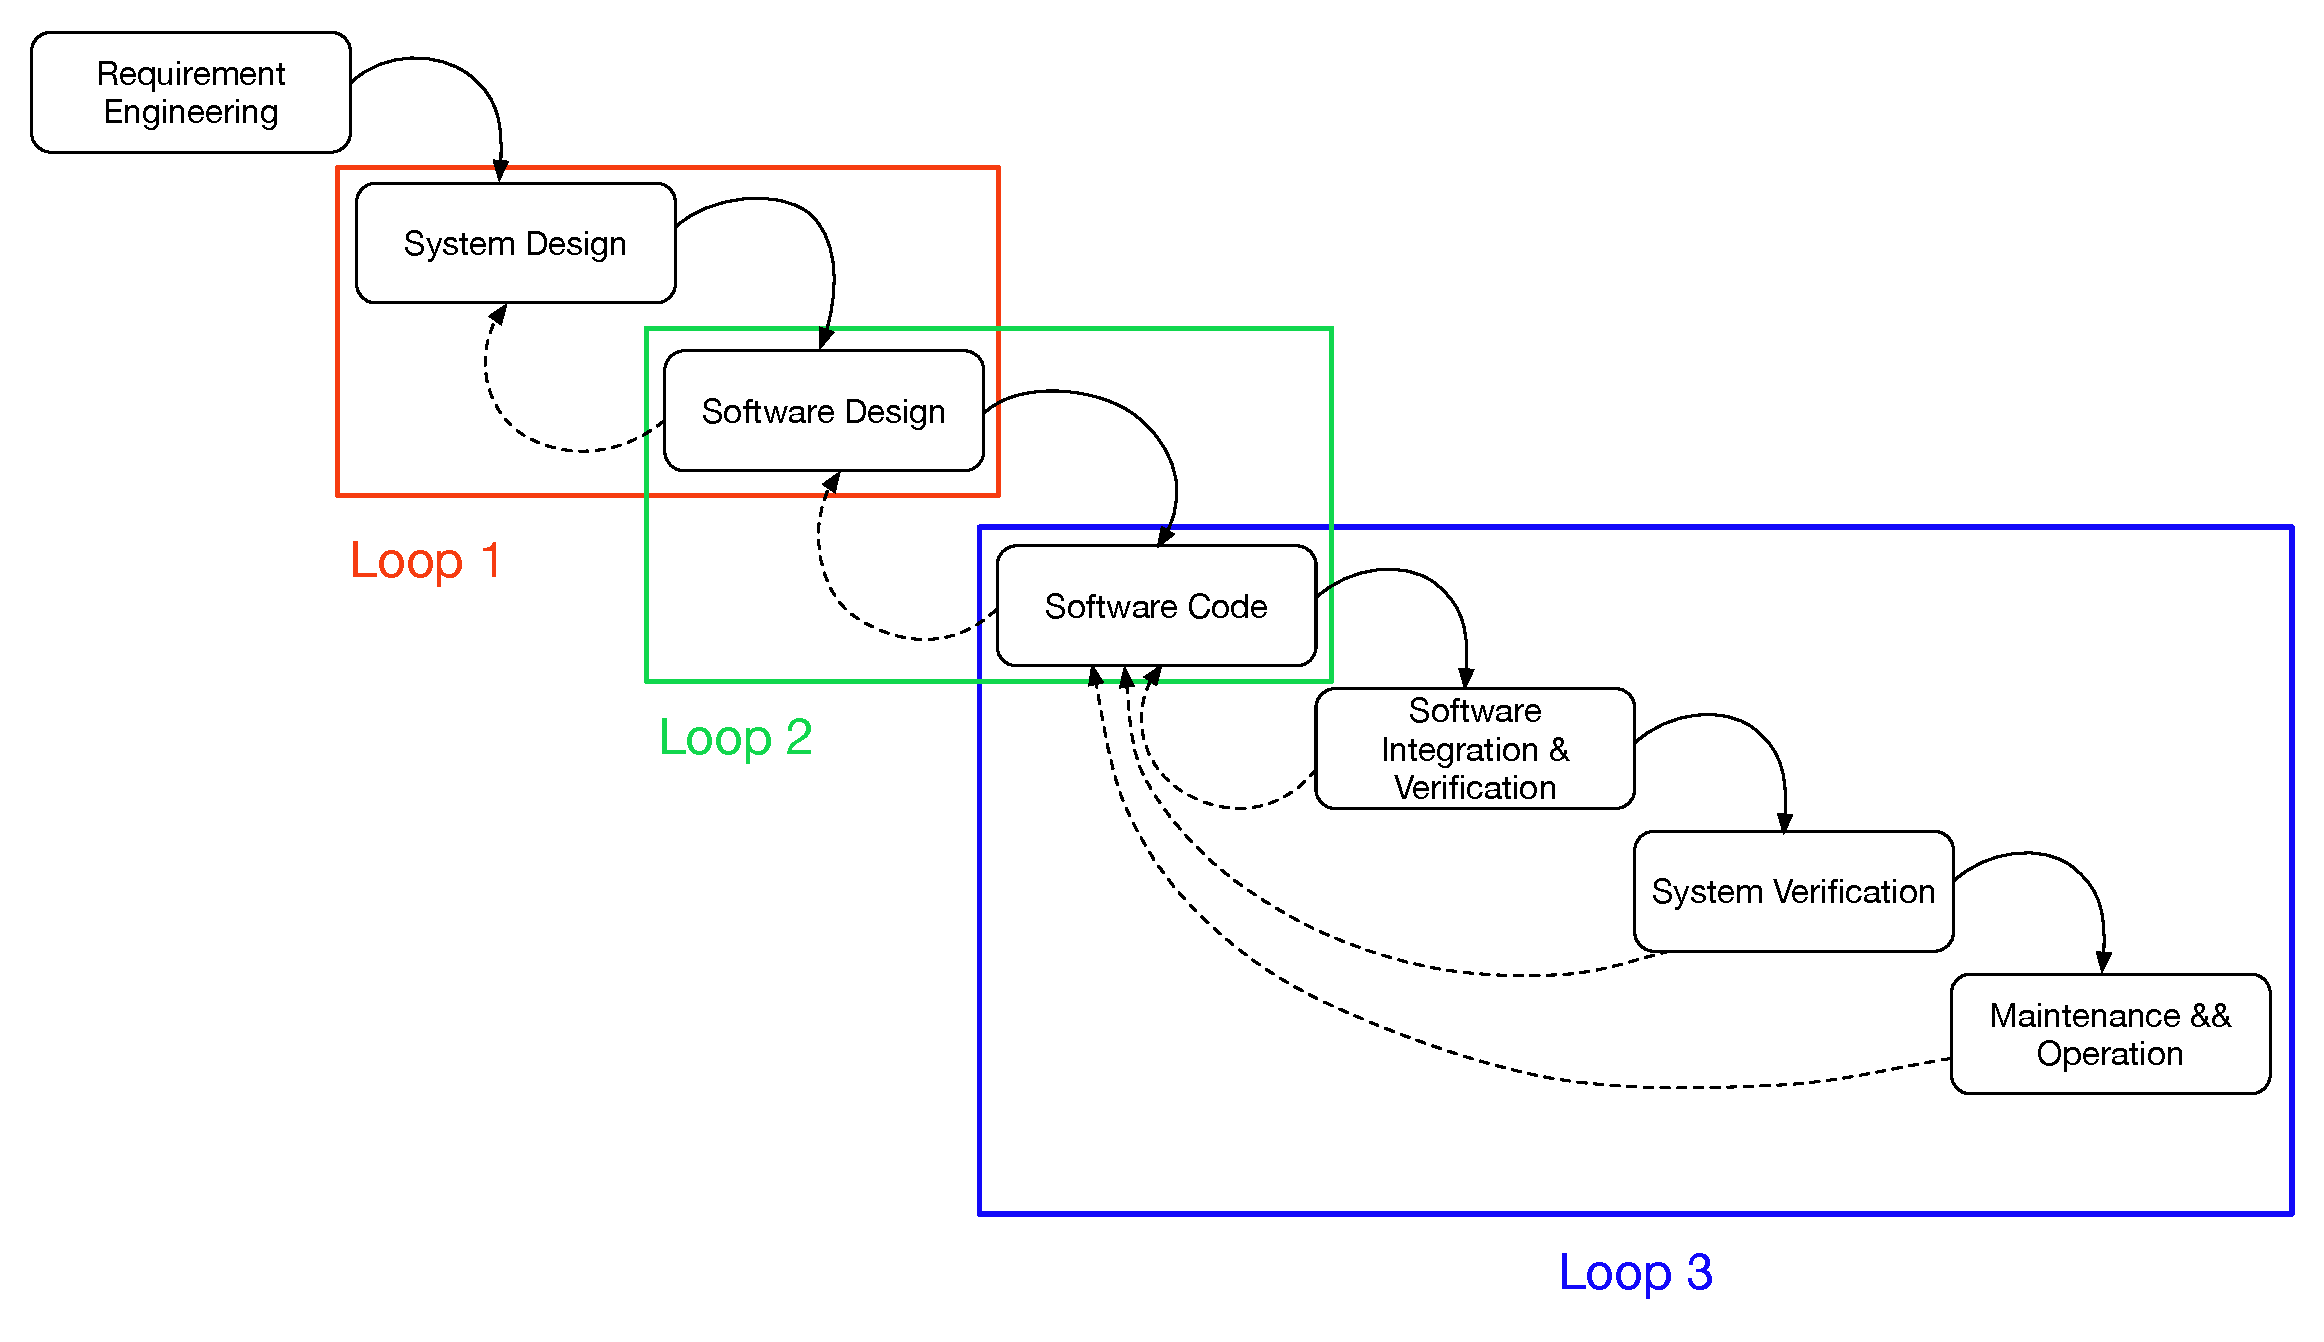
\includegraphics[scale=0.32]{image/campus_waterfall.pdf}
\caption{Campus Waterfall Model}
\end{figure}

In this model, we add four back curved arrows (dashed line) back from certain stage to previous stage and three squares which dicate development loops. The dashed line means the feedback to previous step and we return to the previous stage for improvement or bugs fixing and go along the steps again which finally will be loops. The later loops will be faster than before or even skip some steps since we are more familar to the operations and less modification is needed or even no changes take place. For small projects, this loop will be feasible and useful. At least, in our project, this model helps us go quickly in the development and overcome the disadvantage of original Waterfall Model that only takes a single run through the phase, as well as advantages kept.

 Here we go into details:

1.	\emph{Requirement Engineering}

In this stage, requirements were collected and analyzed in this stage. In this project, the requirements came from sponsors of this project and we further considered them more in an engineering way with the situations might happen such as the increment of users or servers, the cost of the project and the expansibility of the product.

2.	\emph{System Design}

In this stage, we divided the whole development into two parts, the front end system and the back end system according to the requirements. Then another important part, communication between front and back end came out. So, All three parts make up of the whole game.
	\begin{itemize}
	\item For front end, we chose game engine Phaser  combining JS/HTML/CSS to implement all the pages and animation in the game.
	\item For back end, we use a normal game framework, which includes a Nginx reverse proxy server to handle massive request from front end, Tornado servers as application servers to run game instantly. We also planned to use Redis as cache server and mongoDB as database if necessary. We left the cache and database part as an extend development plan since we didn't need them temporarily(more detail in later section).
	\item For communication part, we used JSON to store data(so it can be used in MongoDB or cached in Redis) and transfer message data between front and back end.
	\end{itemize}

3.	\emph{Software Design}

Based on the previous stage, this stage is to further design the software in the framework. State diagram and UML were designed in this stages and all the game logic were split into various code modules to guide the code implementation in next stage. Classes were also designed under the principle of object-oriented programming since we were going to implement this project in OOP way. In this stage we can also go back to previous stage to adjust the system design to make it more feasible to implement since the software or tools we chose might not fully support what we need.

4.	\emph{Software Code}

In this stage, all the codes are implemented under the guide of the UML designed in previous stage and state diagram were used to validate the running result of codes. Also, there is a loop here indicate the coding process will also influence the UML design since some design is not easy to implement so we will modified the UML to  lower the difficulty of coding which also lowers the existence of bugs.

5.	\emph{Software Integration \& Verification}

In previous stage, codes were developed in independent unit and can be tested for its functionality by using unit test. In this stage, unit codes were integrated and tested in a whole by using integrated test to see if all modules cooperate as expected. Feedback still needs to be returned to previous stages for code improvement.

6.	\emph{System Validation}

In this stage, the three parts were to be assembled into a complete entity then we conducted the system test for this software on the hardware we designed before and fed back the bugs or problems to coding stage.

7.	\emph{Operation \& Maintenance}

This stage means we are almost finish this project but we need to do something for further maintenance of our project. We conducted online test by inviting some friends to be the initial users and give us feedback. According to the feedback, we might need to go back to perfect our codes.

The sofaware engineering process is much important for developing a real software involved with engineering technique from design to release so that it can work as expected.

\section{Requirements}
This project is a web-based game design project, so it involves web development techniques and the requirements of this production includes all the fundamental features and some new features the sponsor wants:

1.	allow players to enable a random sequence of spots as well as a periodic, random change of the properties pricing, rents, interests and taxes rates (in both spots and cards);

2.	allow a loyalty program to enable the use of virtual currency with random rules based on existing international alliances programs;

3.	allow new players to join the game as entrepreneurs

4.	allow complexity setting in three levels (e.g., easy, medium, hard) based on rules and different configurations from exploring variabilities on the previous three bullets.

\subsection{Design \& Tradeoff}
To meet the basic requirement and achieve better user experience, we add some new features in this game. However, during the implement process, we encounter many difficulties. We solved some of the difficulties and we did made some tradeoff in this project. The new design and tradeoff shown as follow:

1.	\emph{New Features}

a)	Economic Factor

In the requirement, property value, rent pricing, tax etc. should be set as dynamic value in the new monopoly game. After our discussion, we thought that, randomly change all the value individually may influence the balancing of the game. Therefore, we analogy from GDP or some relative economic index, we introduced Economy Factor(EF) to the Epic-Monopoly. EF act as a global rule which in charge of the change of the price of properties, tax and value of other object. 

For a specific period, EF will change between a certain range, and it will have influence on the rent, pricing of the house, etc. Because of its characteristic, the average value of all property is same. It is seldom for a property devalue every period, which is unfortunate for the owner of this property.

This new mechanism enables the game closer to our real life.

b)	Dynamic Map

The sequence of spot in the Epic-Monopoly will change in a specific period, to repick the fate of players who falling behind. To unify the map, the change of color blocks, stations and utilities will be control by some rules. Therefore, some wired situation, such as successive chance block, will not happened in Epic-Monopoly.

c)	Country \& Alliance

There is no benefit for corporation in the old version monopoly. Therefore, countries and alliances are introduced to the Epic-Monopoly. Every player will assign to one countries and corresponding alliances. The trade and rent between the member of alliances will make discount. And some new event will add to opportunity, to add more fun. In reality, tax and warfare differ depends of country's policy. Therefore, the tax and some of cards in chance and chest will depends on which country the player belongs.

d)	Difficulty Setting

In the old version of monopoly, players can custom some game configuration such as limitation of house etc. However, in the Epic-Monopoly, the old custom configuration is kept, and we introduce difficult setting. Again, to balance the game, the difficulty depends on the fluctuation of the game parameter EF. For example, easy model the EF setting will within 5\% while normal model will be 10\%. 

e)	New Player

Enterprisers can join the game after the game began. However, the enterprisers only able to join when unacquired real estate more than 50\%. And the initial cash of the enterprisers is depended on how many turn the game have begun.

f)	Loyalty Program

Instead of return cash or virtual currency, Epic-Monopoly will make discount for enterpriser. (The effect is same, but simpler) With the time enterpriser enter other's spot, the rent of the spot to this enterpriser will decrease. Same rules for prison. With the time an enterpriser bail from the prison, the price will increase, which is same as reality (The more in to prison, the more bail fee it must paid).

2.	\emph{User Interface Design}

a)	UI Design

To pay our respect to the old version monopoly which is created in 1903, the key design principle of Epic-Monopoly UI is classic. The design of card and chessboard are old fashion. Despite those, we used wooden background which represented the wooden table people used to play in. 
\begin{figure}
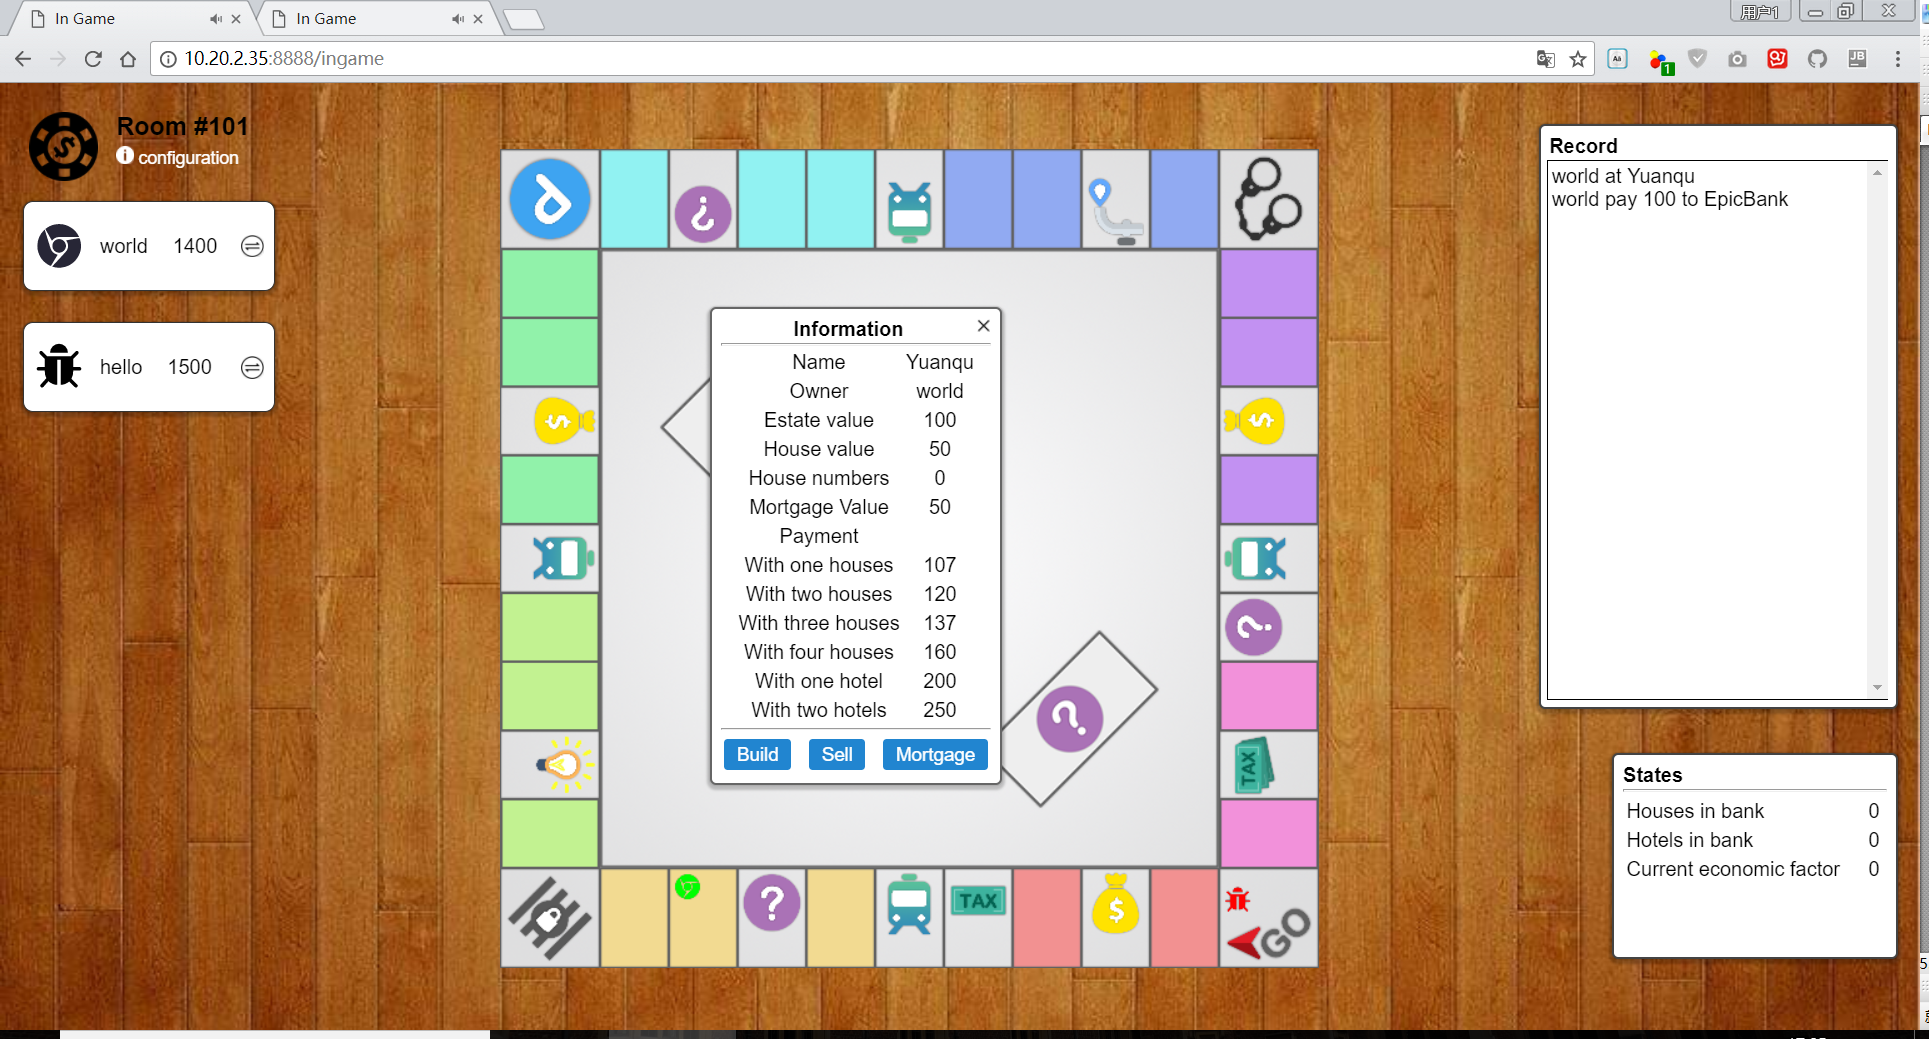
\includegraphics[scale=0.32]{image/ingame2.png}
\caption{Management page}
\end{figure}

More about UI are attached in Appendix II-UI.

b)	Animation

Epic-Monopoly, as a web-based game, user want to open it within seconds. We have to tradeoff of our expectation about animation and $3$D chessboard. In the current design, we used $2$D chessboard and simply movement animation. For the final implementation, we may switch to $2.5$D, which known as fake $3$D.

3.	\emph{Game Logic Design}

a)	Object Oriented

Epic-Monopoly has many objects in the game which can be extracted to classes. Thus we designed the game logic in object-oriented way. We designed with as less as possible classes by using inheritance mechanism and polymorphism. The classes have no overlapped in its function, greatly simplified our codes, and also made the codes much easier to maintain. The relations of the classes the code are constructed based on the state diagram. 

The state diagram are attached in Appendix I-State Diagram.
The UML are follows in Appendix I-UML.

b)	Safety

The game logic runs only on the server, and both the front and back end will check the details and results of the game, ensuring possibility for players to cheat.

4.	\emph{Server Design}

We divided server to three parts, request, gaming room and communication. The request part takes in charge of analysing the request from user and act corresponding operation, like built room or enter room. If all users agree to start game, the server will build a process for the gaming room to start the game logic. For the final part, we defined the JSON format to transmit data from game logic to user interface. We use WebSocket to implement the communication part. For the further implementation, we will use MongoDB to store user information and data of every game and Redis to cache data if necessary. Those data will be very helpful for change the gaming parameter to have better game balancing. For consideration of scalability and concurrence, we plan to use Nginx as reverse proxy server to distribute requests from front end to distributed servers which provide the software scalability and provide a better concurrence.

\section{Implementation}
\subsection{Team assignment}
There are five developers in our team: two for back end development, two for front end development and the other one applied the communication of back end and front end. In design stage, all five developers designed the game logic together. Then one of the back end developers and communication developer drew the UML and state diagram. Later two back end developers confirmed the JSON format for data transmission together. In implementation stage, simultaneously, one front end developer designed the UI and the other front end developer implemented the animation in the game and web pages while two back end developers implemented the game logic.

However, as the project processed, it was difficult to finish the task independently. There are some time we worked together on same part of work, especially the front end part involved with much work that even dragged our progress. 

\subsection{Platform choices}
\subsubsection{Back end}
 Back end is implemented by Python $3.6.4$ with Tornado framework.
 
1.	\emph{Object Oriented}
 
Epic-Monopoly is designed by object-oriented ideas. At the beginning, it took us over one week to design the UML which further helped us a lot during the implementation. The main game logic is divided into several parts and every part is defined by some super classes. For example, the "Block" class is the super class which represents all the block in the chess board. The "Block" can be further divided to "Asset" which represents the properties in the game, "CardPile" which represents the "Chance" and "Chest" block in the chess board. And those sub-classes can be divided into even smaller class, "Asset" can be divided into "Estate", "Utility" and "Station", which are the three main properties that players owns in during the game. Every sub-class have their own game logic and attributes but share many same attributes like "name", "id" and "position". The benefits of using object-oriented design, on the one hand can reduce the lines of code, on the other hand, let us focus more on the difference between classes. Also, it is very convenient to debug and further maintain as well. At the end of this project, we found a extremely wired bug. After analysis and tests on it, we realized it happened in the common codes among "Estate", "Utility" and "Station", thus we are able to find the mistake and repair it.

Moreover, there are many similar methods used in the program. For example, payment, is used by many objects to process a trading case. Therefore, we extract this kind of methods to a file named "operation", and almost all classes will import this module since they need the common method. It will also prevent the re-import problem. We do the same procedure when we designed the "messenger" class again. It embedded all the methods about communication between client and server.

2.	\emph{Speed}

Epic-Monopoly is a web-based game. User are not willing to wait for several seconds or even minutes for the initialization of a game. While we loading the files from server, the user can use those time to create a room or join a room. The loading time much tougher to observe. Also, we use CDN to delivering the data quickly, which speeds up the initialization and reduces the pressure of our server.

3.	\emph{Safety}

The game logic runs only on the server, and both the front and back end will check the details and results of the game, ensuring possibility for players to cheat. The data transmitted on the link can be encrypted if use HTTPS.

4.	\emph{Balancing}

There are many feature introduced in the new monopoly, to balance the game and maximize the happiness of players. Epic-Monopoly was tested to balance the new features and original game settings.

\subsubsection{Front end}
Front end includes \textbf{page design} and \textbf{animation design}. 

For \textbf{page design}:

There are two pages in Epic-Monopoly. The first is login page and the second is game page. 
	
In login page, we use a \textless canvas\textgreater\; element as a container, a \textless form\textgreater\; to collect players' personal configuration (nickname and avatar) including an \textless input type="text"\textgreater\; element and a \textless select\textgreater\; element. 

Then if player chooses to create a room, a hidden \textless div\textgreater\; element will be displayed, which contains another \textless form\textgreater. That \textless form\textgreater\; contains an \textless input type="text"\textgreater\;element, several groups of \textless input type="radio"\textgreater\; elements and \textless input type="checkbox"\textgreater\; element, to set up all configurations of the new room. After player confirming his settings, the function \emph{createRoom} will be called. It then calls \emph{getPlayerJson} and \emph{getRoomJson} to obtain all settings of the player in JSON form and sends a HTTP POST to transfer the aggregated JSON to the server. Then read the JSON returned by the server and stores them in sessionStorage, and finally let the window jump to the game page.

And if player chooses to join a room, the function \emph{getRoomList} will be called. It sends a HTTP GET request to the server to get all information of existing rooms at that time, then reads the JSON returned by the server and adds data into a \textless table\textgreater\; element in another hidden \textless div\textgreater\; element, and finally displays the hidden \textless div\textgreater\;. Then player can join any room that is still not filled by $6$ players. After that function \emph{joinRoom} will be called. It then calls \emph{getPlayerJson} to obtain all settings of the player in JSON form and also the room whom player chose to join and sends a HTTP POST to transfer the aggregated JSON to the server, then read the JSON returned by the server and stores them in sessionStorage, and finally lets the window jump to the game page.
	
The game page is divided into three parts: left part, mid part and right part. The left part contains two \textless div\textgreater\; elements: one to displays room information, another to display all players and their basic information in the room. Each player is displayed in a \textless div\textgreater\; elements containing an \textless img\textgreater\; (to display avatar), two \textless span\textgreater\; (to display player's name and cash) and an \textless a\textgreater\; (as a trade button). The player \textless div\textgreater\; elements are all hidden and will be displayed when a new player joins the room. 

The mid part contains a \textless button\textgreater\; to start gaming and a hidden \textless div\textgreater\;. When player presses the start button and the room is permitted to start a game, the button will be hidden and the hidden \textless div\textgreater\; containing the chessboard will be displayed. 

The right part contains two \textless div\textgreater\;, record and states. The record contains an inner \textless div\textgreater\; to display all record of the game and the states contains a \textless table\textgreater\; to display some dynamic data during the game.


For \textbf{animation design}:

1.	 sessionStorage: store room id, users' id, users' avatar. And these data will be cleaned when the browser closed.

2.	Chessboard part:

	Chessboard is a canvas, there are two main parts in chessboard to implement the animation design: \emph{preload} and \emph{create}. We put \emph{update} part into the \emph{create} part since we need JSON data when initializing the chessboard.
	
	We only use \textbf{Phaser} game framework in our project.
	\begin{itemize}
		\item The first part is preload. In this part, we load our elements including images and spritesheets. We also new a \textbf{WebSocket} object here to build communication with back end.
		\item The second part is a function: \emph{WebSocketTest}\\
		We implement the actions according to the JSON files sent by back end
		\begin{itemize}
			\item Init:
			\begin{itemize}
				\item Create the part of chessboard which will not change during the game. Such as the four corners , chest blocks and chance blocks.
				\item Create the rest part of chessboard according to the JSON file, such as estate, station and utility.
				\item Create the players on the "Go" block.
			\end{itemize}
		\item Update:
		\begin{itemize}
			\item Update the block information
			\item Update the players' information including their position, cash 
			\item Update estate, station, utility information
			\item Bank information
			\item Economic Factor
		\end{itemize}
	\item Hint:
	\begin{itemize}
		\item Show message on the screen last two seconds.
	\end{itemize}
		\end{itemize}
		\item  Some isolated functions:
		\begin{itemize}
			\item create\_house: creates houses or hotels according to the house number of the block information
			\item listener \& show\_block\_infoContect: shows the corresponding information window(estate information window, ) when click the block sprite
			\item roll\_dice: control dice rolling action
			\item mortgage: send a mortgage request when click the mortgage button
		\end{itemize}
	\end{itemize}
\subsubsection{Communication}
Our server is based on \textbf{Tornado} which is a Python web framework and asynchronous networking library. Its two features are what our game program needs. Tornado deals with all requests from client in our present architecture. Server will monitor all room members (clients) if their links are alive. If not, the server will destroy the room, close the socket, empty the memory for the rest of other games. 

The program doesn't have an account management system, and we consider that a player who creates or joins a room is ready for starting games. We also allow that players join a game which is ongoing, but follow the rules on initial cash for balancing the game.

If room owner creates a room, the server will not create a game immediately. Until the room has enough players and one of them clicked “start game” the server will create a new game instance in another threading. Also, the server threading communicates with the game threading through pipe, which notifies the game threading the clients activities. The game message uses a queue to preventing from blocking on received or sent messages.

In the further development, if take the scale of multiplayer game, single Tornado server cannot bear. So, we can add the Nginx server as reverse proxy server to balance the server pressure with distributed Tornado servers.
\subsection{Design changes}
We recently change our design of front end part.

1.	Add a loading page

	Before loading all the items from the server, we add a loading page to show the rate of progress.

2.	Add creative room and join room layout on the login page

	We do not design the create room and join room layout in our first design version. 

3.	Change left part of player list in game page

	The in game page does not show anything before all the players click the start game button.However,it may not accord with the formal condition because the players do not know how many players are ready in the room and who are the other players. So we change the trigger function of player list, the player list may first show the player his/her own information and add the other players' information when then the other players clicking the start game button. 

4.	UI style

	We change the color schemes to make the chessboard more striking while implementing our UI design.

\section{Verification \& Validation activities \& outcomes}
At the beginning, we thought about what this game flow should be like, and determined what programming language and framework should we use. Then, we drew a state diagram to describe it. At the same time, we also drew a class diagram which shows the skeleton of Epic-Monopoly class should be like such as the attributes, the functions and the relation of the classes.

The UML can help other members of our team understand the structure of the program as soon as possible, and if we modify it in the future, UML can explain it well for us. However, the most important is UML explain clearly the game's complex logic, multi-level state transition. Whenever we implemented the code, we would not get lost in the game logic.

We verified our game's validation and usability in modules. Each module has several test cases. After we finished all game logic modules, we assembled it into an integral game logic and verify whether each module works together smoothly.

Firstly, we tested the game logic on our local server. Then we added commutation module and put it on to web server. We test it on a prototype website without game UI, which shows all web socket works well. Finally, when the UI part was gradually finished, we integrated both front end and back end to ensure that both ends cooperate as expected.

\section{Implementation operation}
When we implemented our design, we encounter some frustrations which are caused by bad design model due to not considered before. So, our UML have enriched and rebuilt the details several times to achieve the ideal goal.

Taking commutation part as example, we firstly test whether poll to get information from server is a good idea. We found that it is not. Because polling means server passively sending the information to the client. If server has some new game response, this will not be send until next polling. Then we test implementing connection over WebSocket, which can exchange information from both sides and have a great multiplex feature.

\section{Post-mortem Analysis}
This project is to develop a novel monopoly game with more flexible rules and mechanisms. Different from traditional local software entity, this project is web-based which means a different design from original monopoly version like typical V$5$. 

The design of project is not finished at a time but modified many times since we have less experience and knowledge on design. The design of architecture is very hard at beginning even though we had played the original game for some times. After referencing some engineering architecture we finally designed the architecture.

The coding of back end was smooth since we both follow a same coding style much like PEP$8$ and we did not encounter much problems when conducting integrated test. However, peer view and collaborative programming are necessary sometimes so as to keep a high and similar code quality.

Besides, the communication between front end and back end is a crucial part and we need to consider from both ends. It was the first time for us to design such thing so what we paid more attention to the data transmission, JSON here helped us a lot.

Test are identical difficult since this the turn-based game so when and where the imperceptible bugs might happen we can not know and those bugs are usually unrepeatable with the random result of dices. So test should not only involves with correct methods but also enough patience.

And some other engineering situations are need to be take into consideration like the scalability, concurrence and security.
\section{Lessons}
This is the first time we've tried such a complicated project. We had to learn many things in order to accomplish the whole project. It's to develop a software but not to realize an algorithm or solve a specific problem. It's about designing rather than just coding. So more aspects about engineering should be taken into consideration before and during coding. There're mainly two lessons we've learned from this project. 

The first is teamwork. We should reach an agreement on an appropriate work division and how to integrate everyone's work before starting coding. Many important fundamental structures should be settled as early as possible to avoid recoding afterwards. We should combine the whole project from time to time to check if there's inconsistencies.

The second is timing. We haven't arranged a schedule properly and completely as well as strictly observe it. In this case it's hard to perfectly finish the project in time, or we will have to keep coding day and night during some days. On the contrary, everyone should guarantee his/her own portion can be finished on time and try his/her best to not be a drag on others. 

\section{Others}
We had made some new friends through this project and the team became more tacit. We gained a lot of software design and development experience. We also learned some new tools, software and frameworks.

%uncomment follwoing to use refrence
%\begin{thebibliography}{99}

%\bibitem{gonzalez2012} Jonay I. Gonz\'{a}lez Hern\'{a}ndez, 
%Pilar Ruiz-Lapuente,	
%Hugo M. Tabernero,	
%David Montes,	
%Ramon Canal,	
%Javier M\'{e}ndez	
%and Luigi R. Bedin,
%{No surviving evolved companions of the progenitor of SN1006},
%Nature, {\bf 489}, 533-536 (2012).

%\end{thebibliography}
\section*{Appendix I-State Diagram}
\begin{figure}[H]
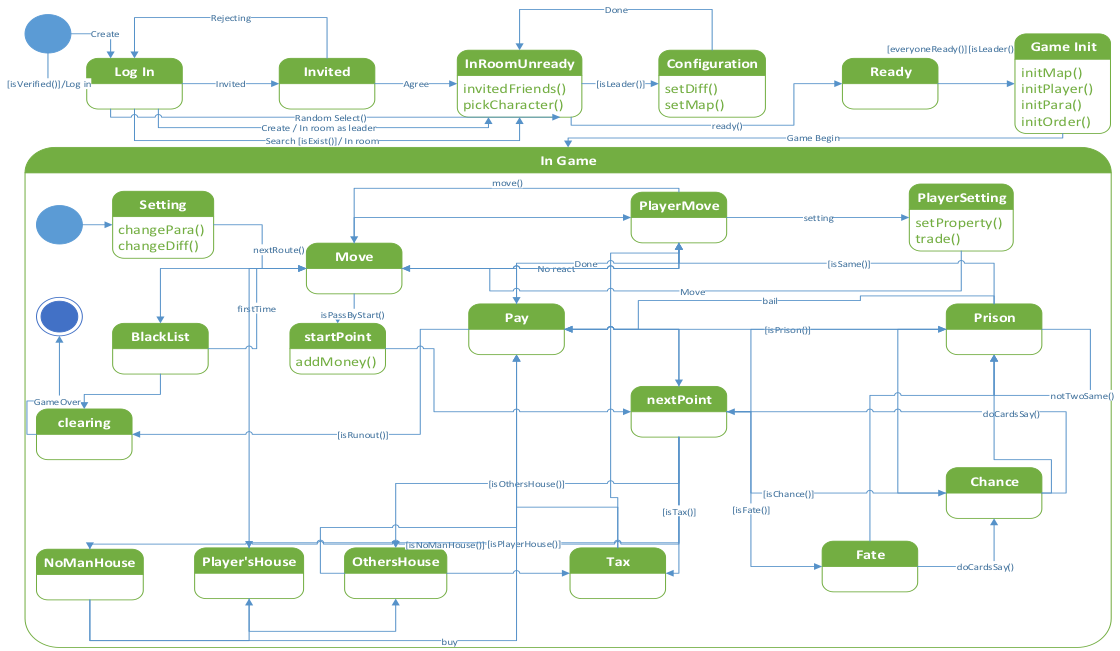
\includegraphics[scale=0.70]{image/state_diagram.png}
\caption{State Diagram}
\end{figure}

\section*{Appendix I-UML}
\begin{figure}[H]
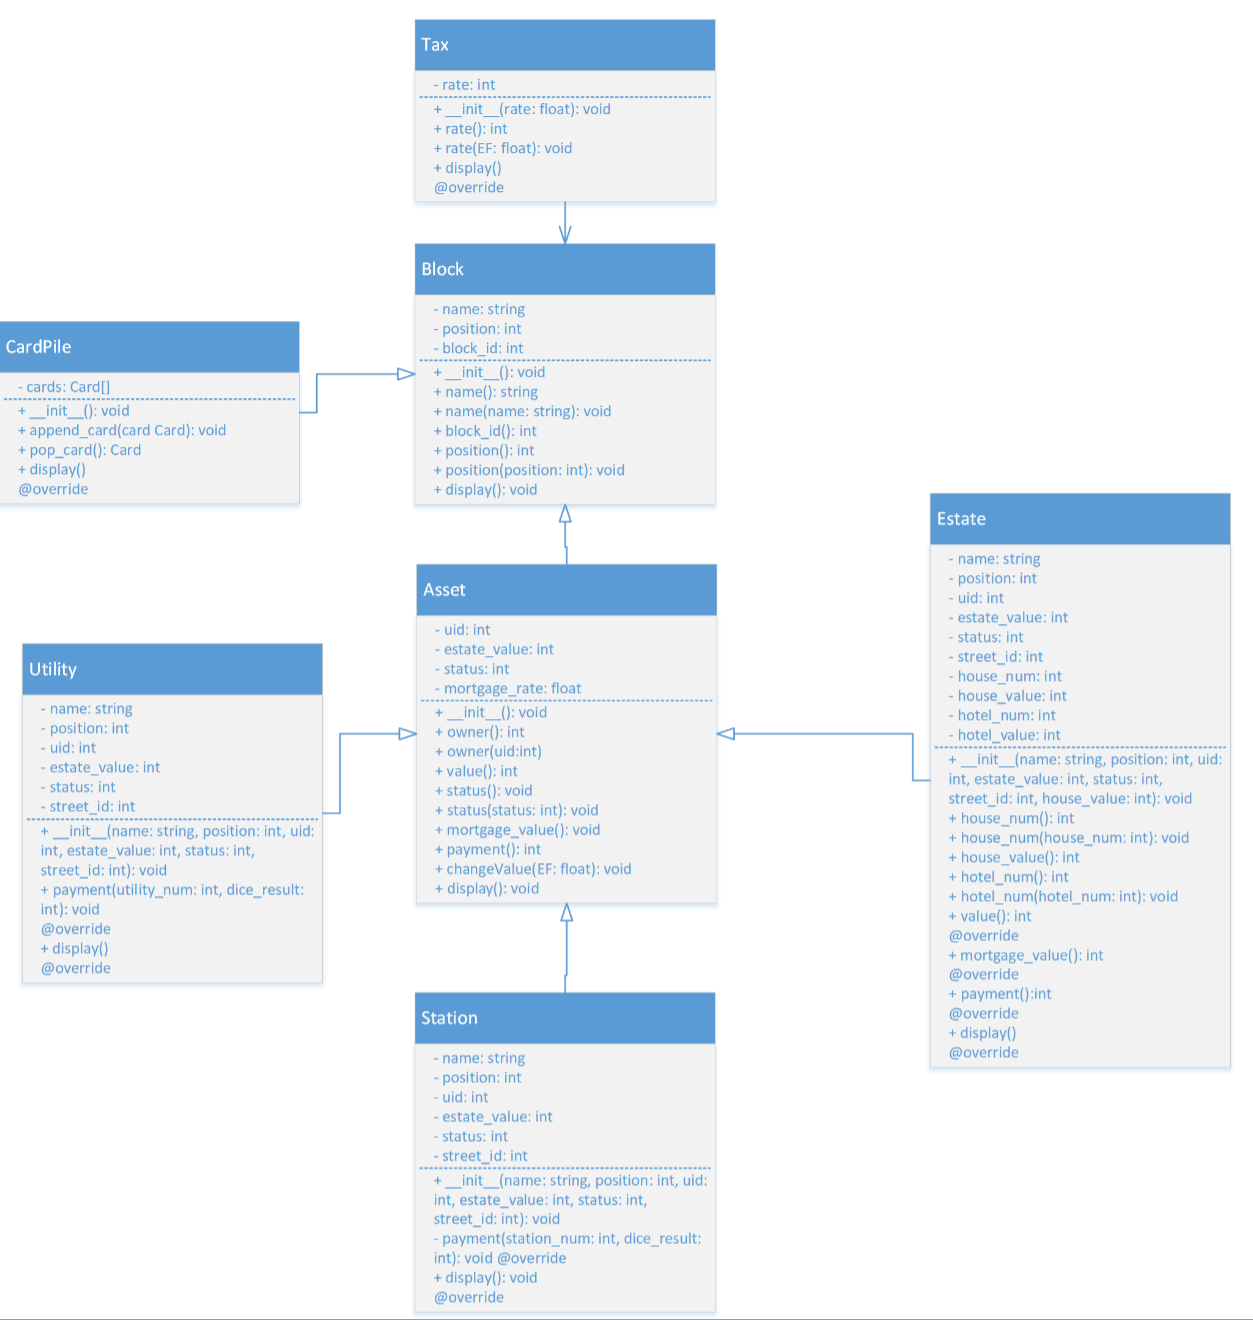
\includegraphics[scale=0.8]{image/Block.png}
\caption{Block}
\end{figure}
\begin{figure}[H]
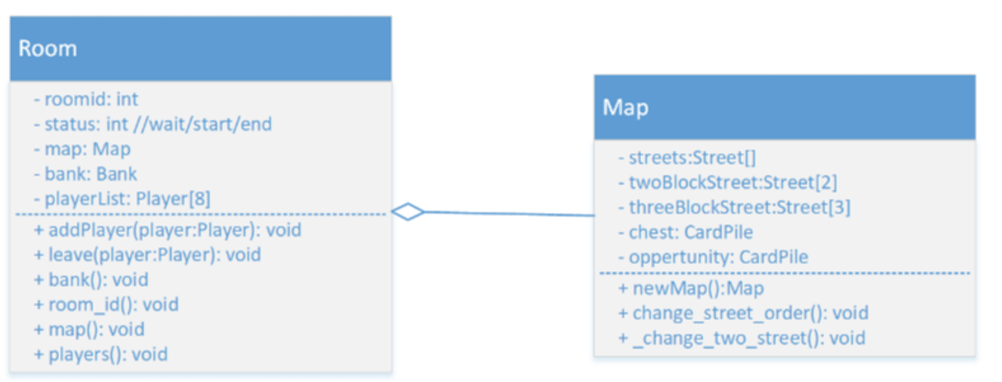
\includegraphics[scale=0.7]{image/roomandmap.png}
\caption{Room \& Map}
\end{figure}
\begin{figure}[H]
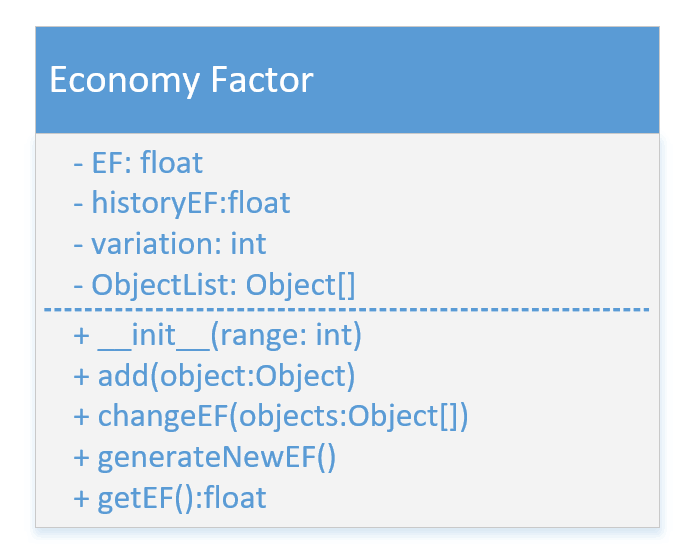
\includegraphics[scale=0.22]{image/ef.png}
\caption{Economy Factor}
\end{figure}
\begin{figure}[H]
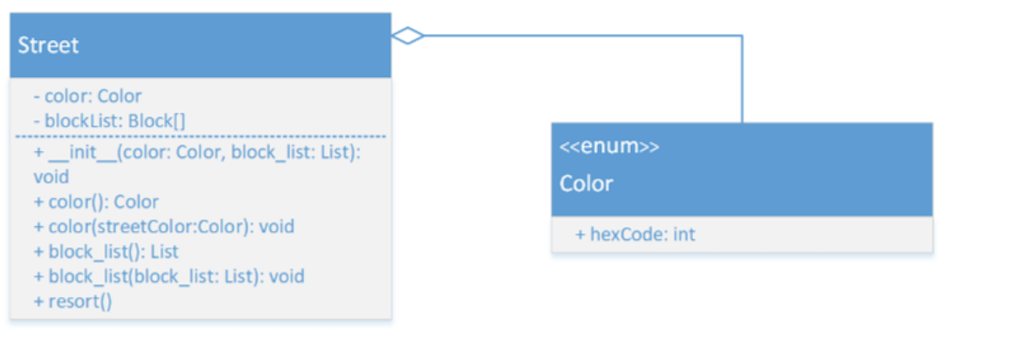
\includegraphics[scale=0.7]{image/street.png}
\caption{Street}
\end{figure}
\begin{figure}[H]
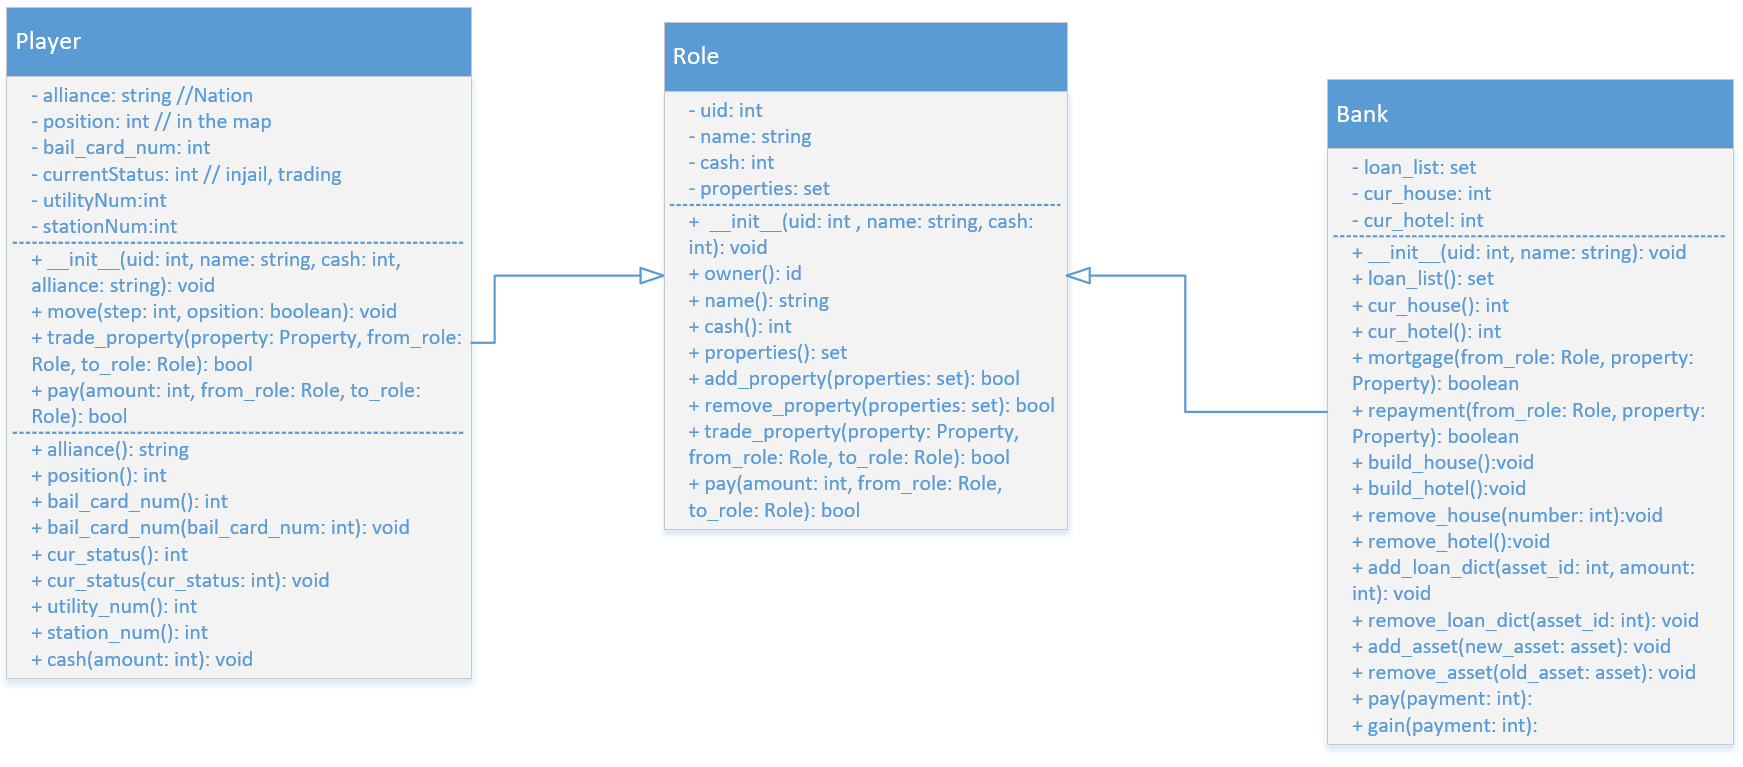
\includegraphics[scale=0.22]{image/role.png}
\caption{Role}
\end{figure}
\begin{figure}[H]
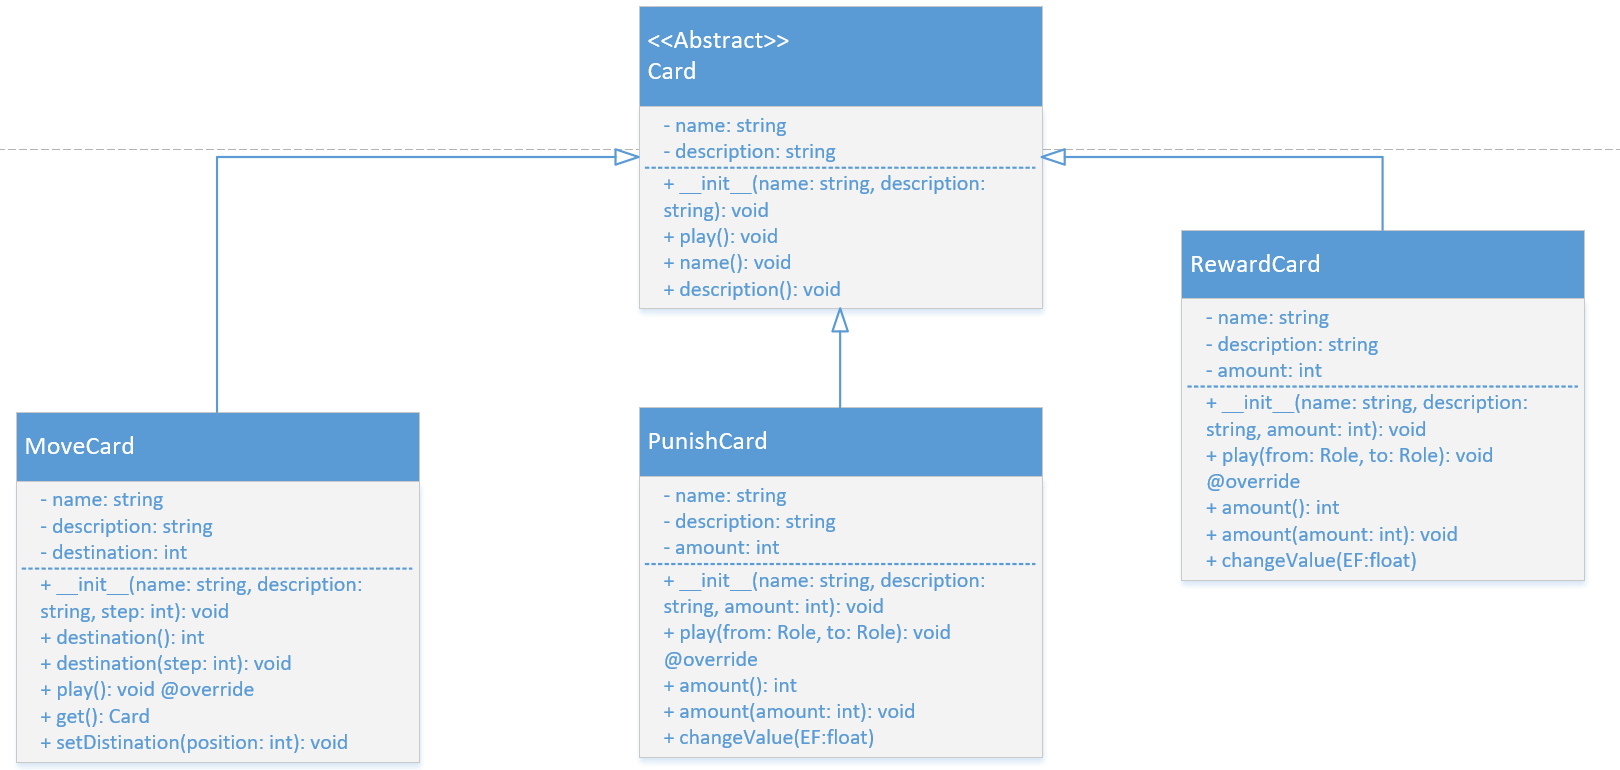
\includegraphics[scale=0.22]{image/card.png}
\caption{Card}
\end{figure}

\section*{Appendix II-UI}
\begin{figure}[H]
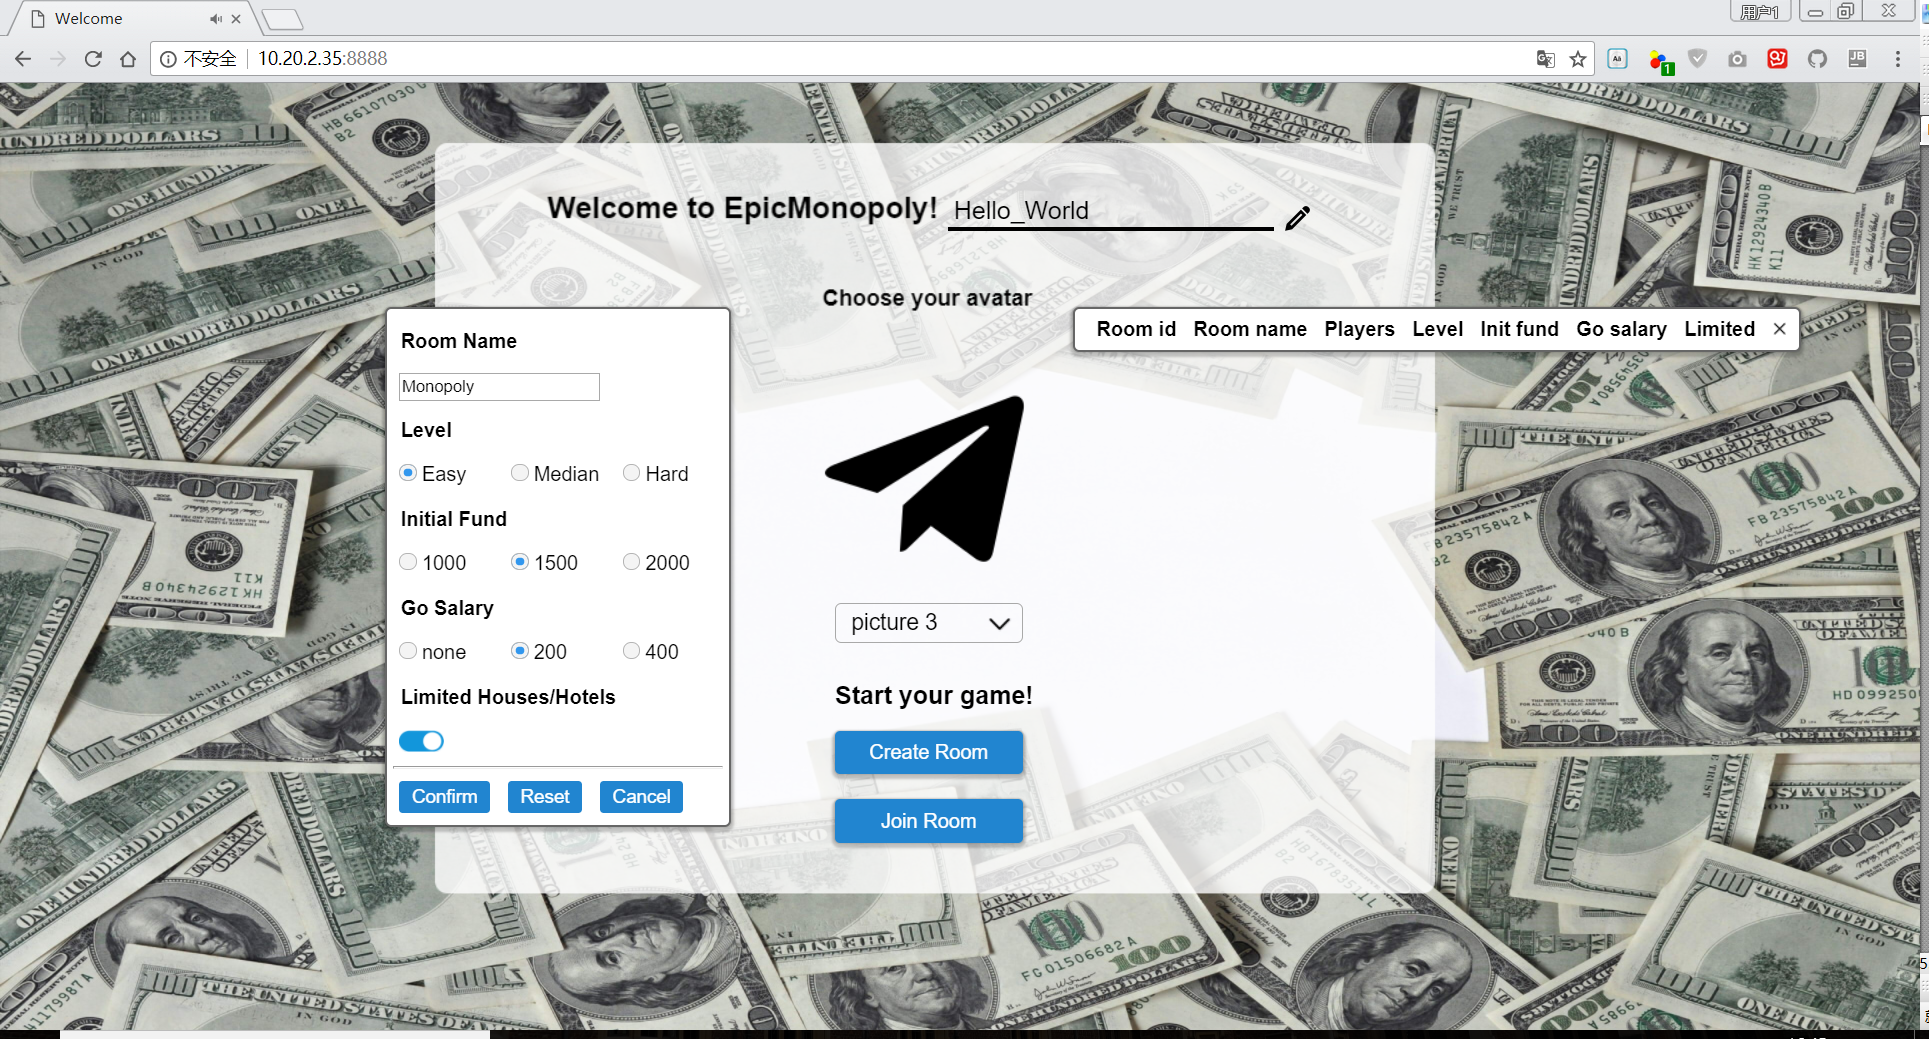
\includegraphics[scale=0.32]{image/login.png}
\caption{Settings}
\end{figure}
\begin{figure}[H]
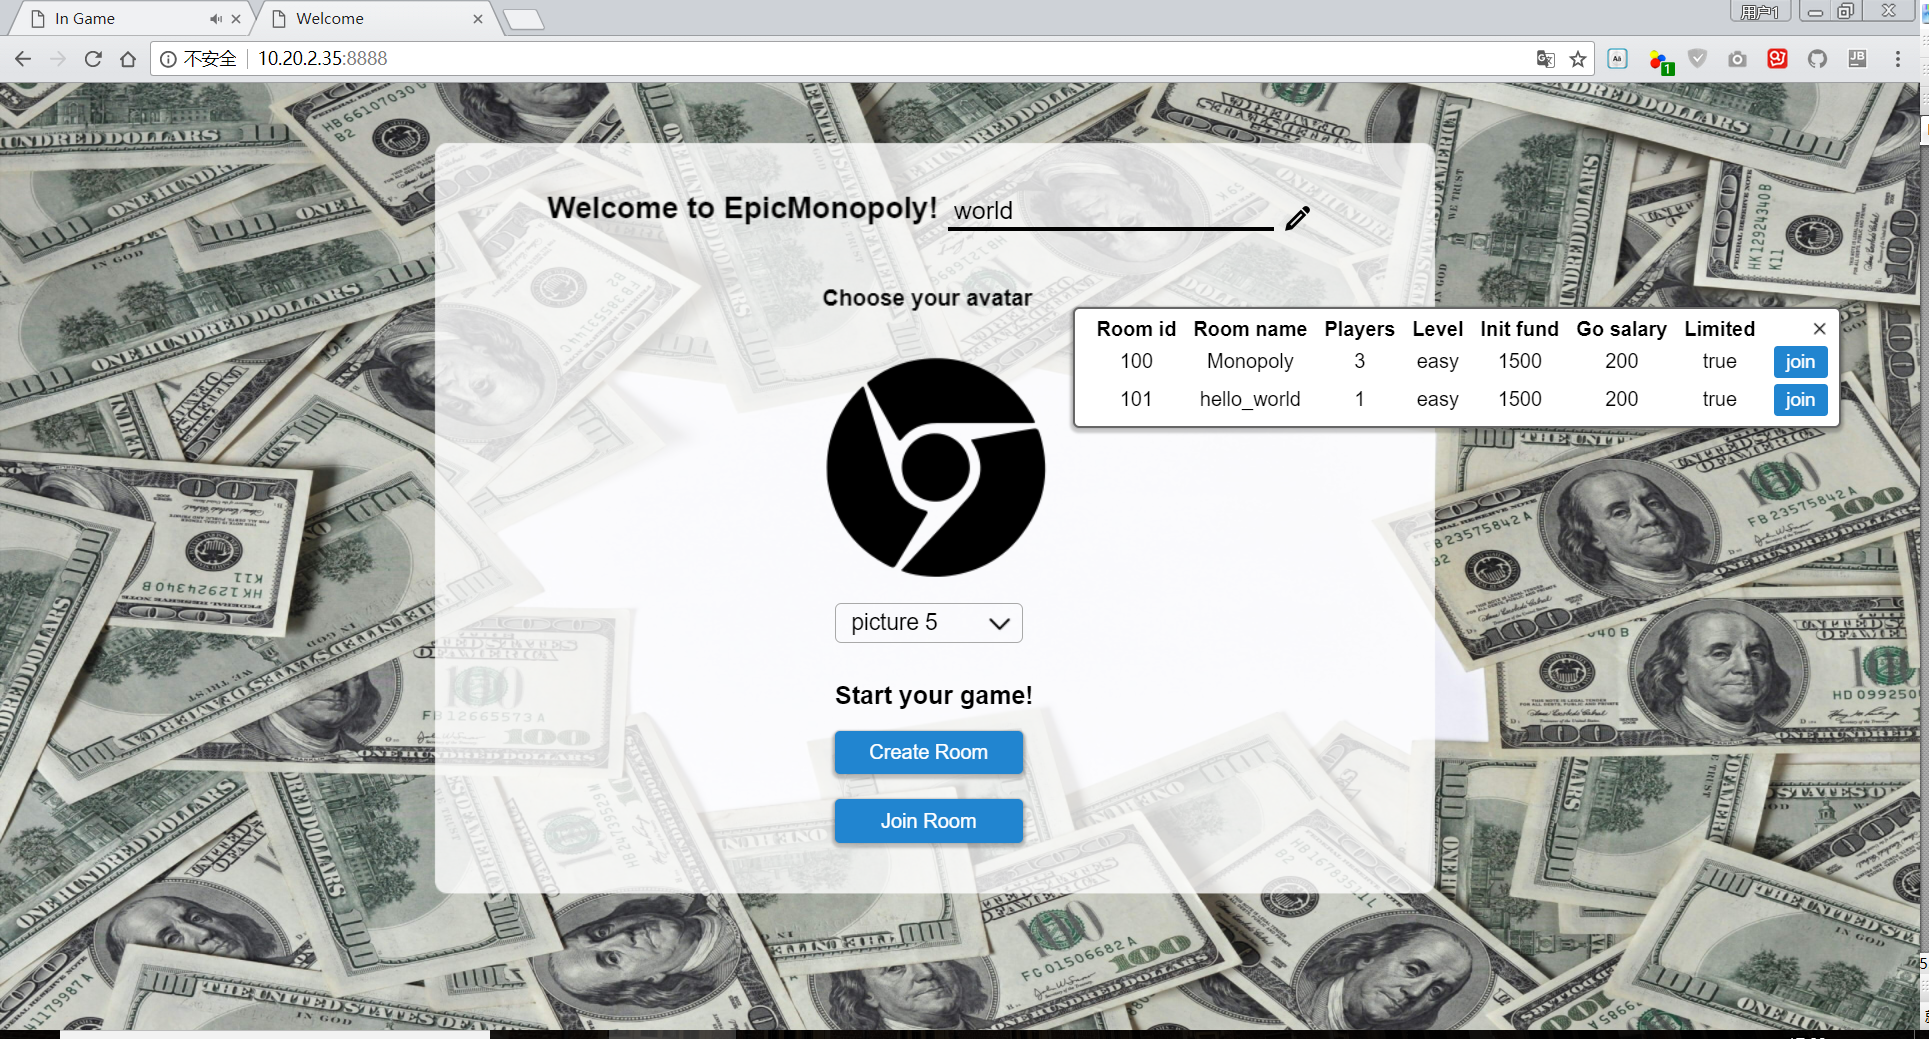
\includegraphics[scale=0.32]{image/login1.png}
\caption{Room List}
\end{figure}
\begin{figure}[H]
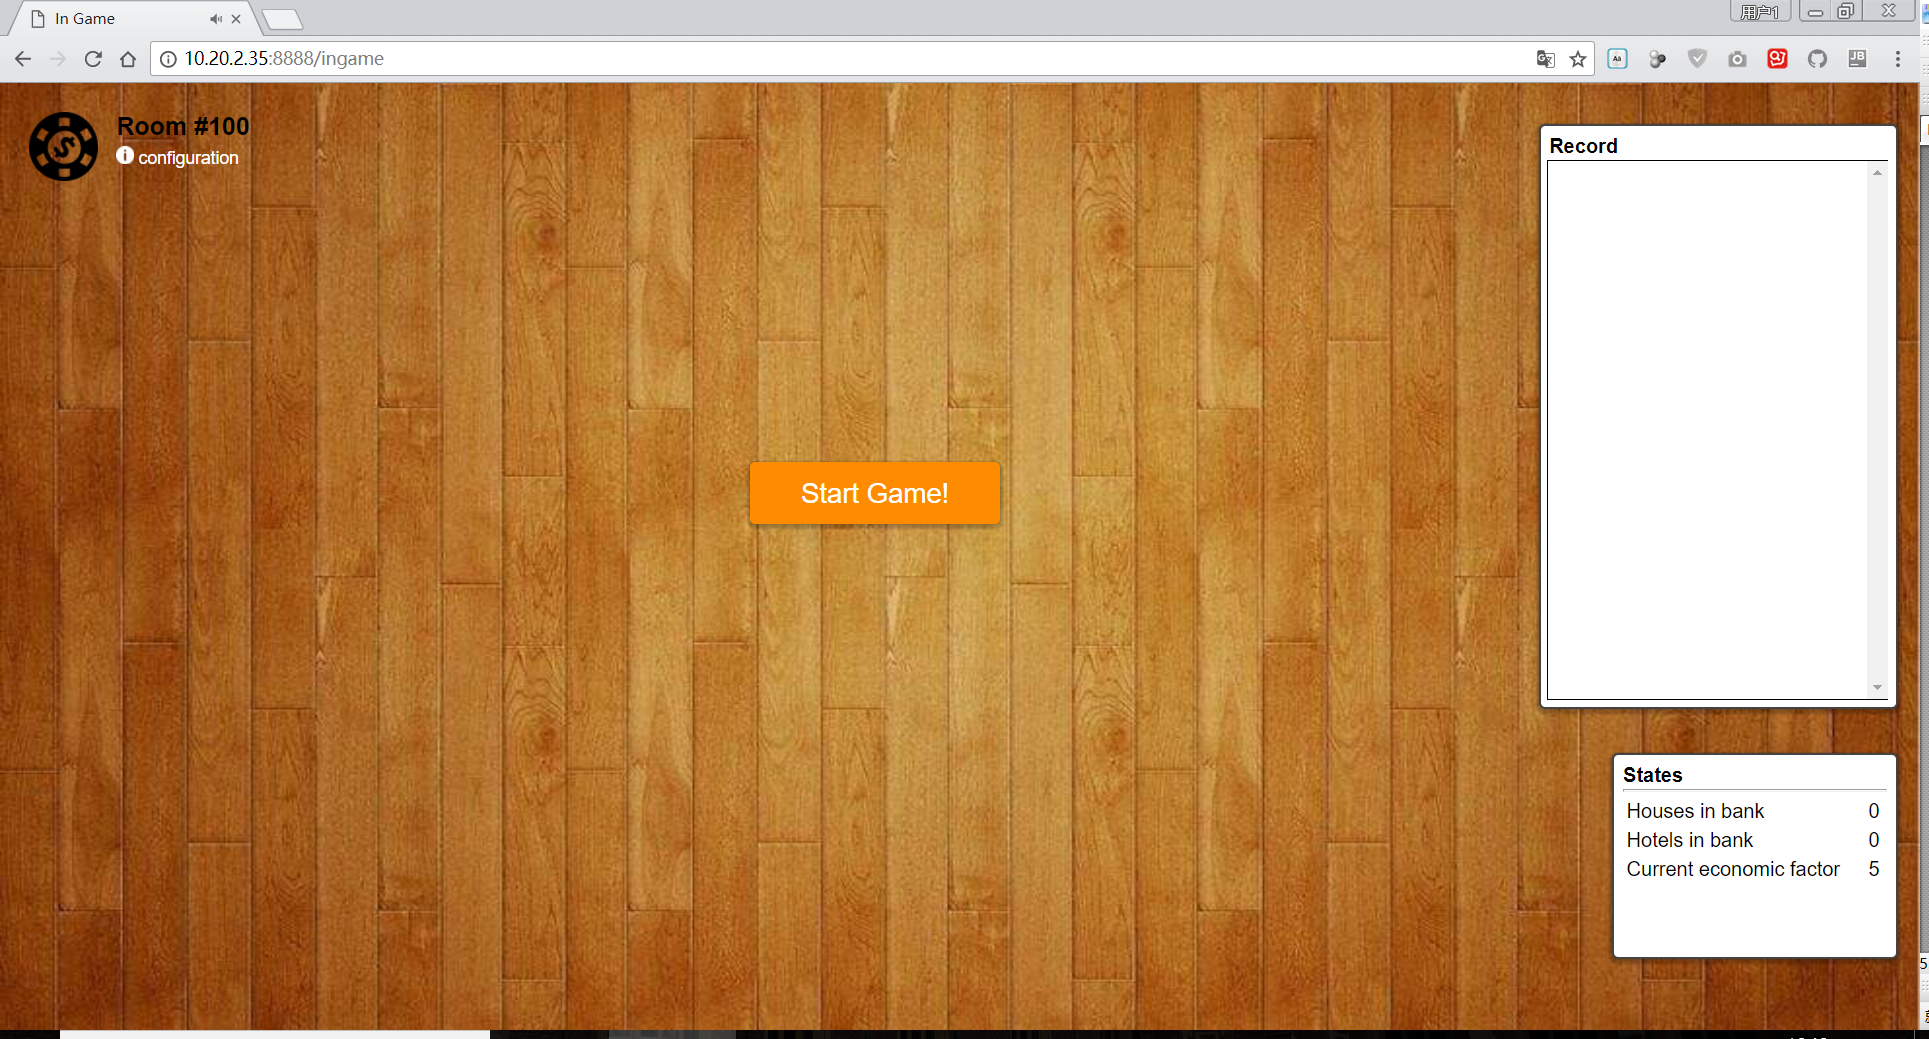
\includegraphics[scale=0.32]{image/start_game.png}
\caption{Start page}
\end{figure}
\begin{figure}[H]
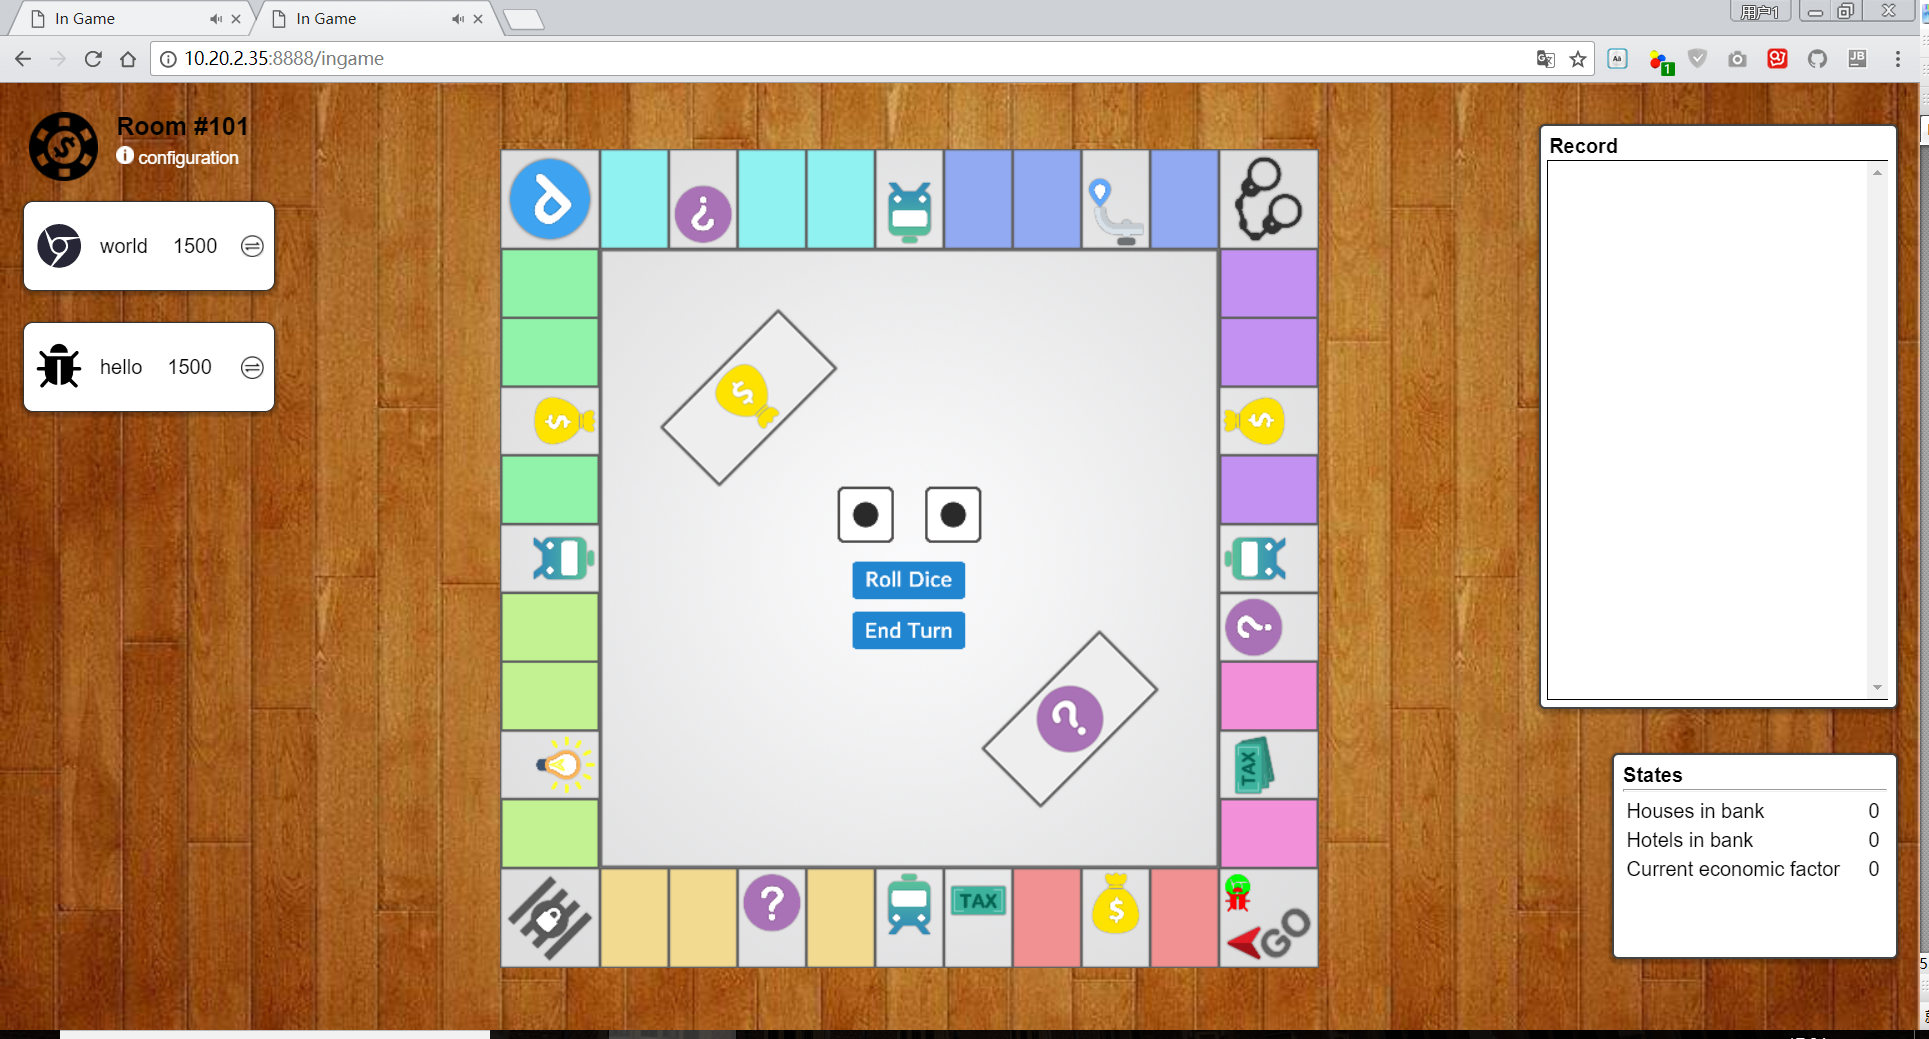
\includegraphics[scale=0.32]{image/ingame1.png}
\caption{Main page 1}
\end{figure}
\begin{figure}[H]
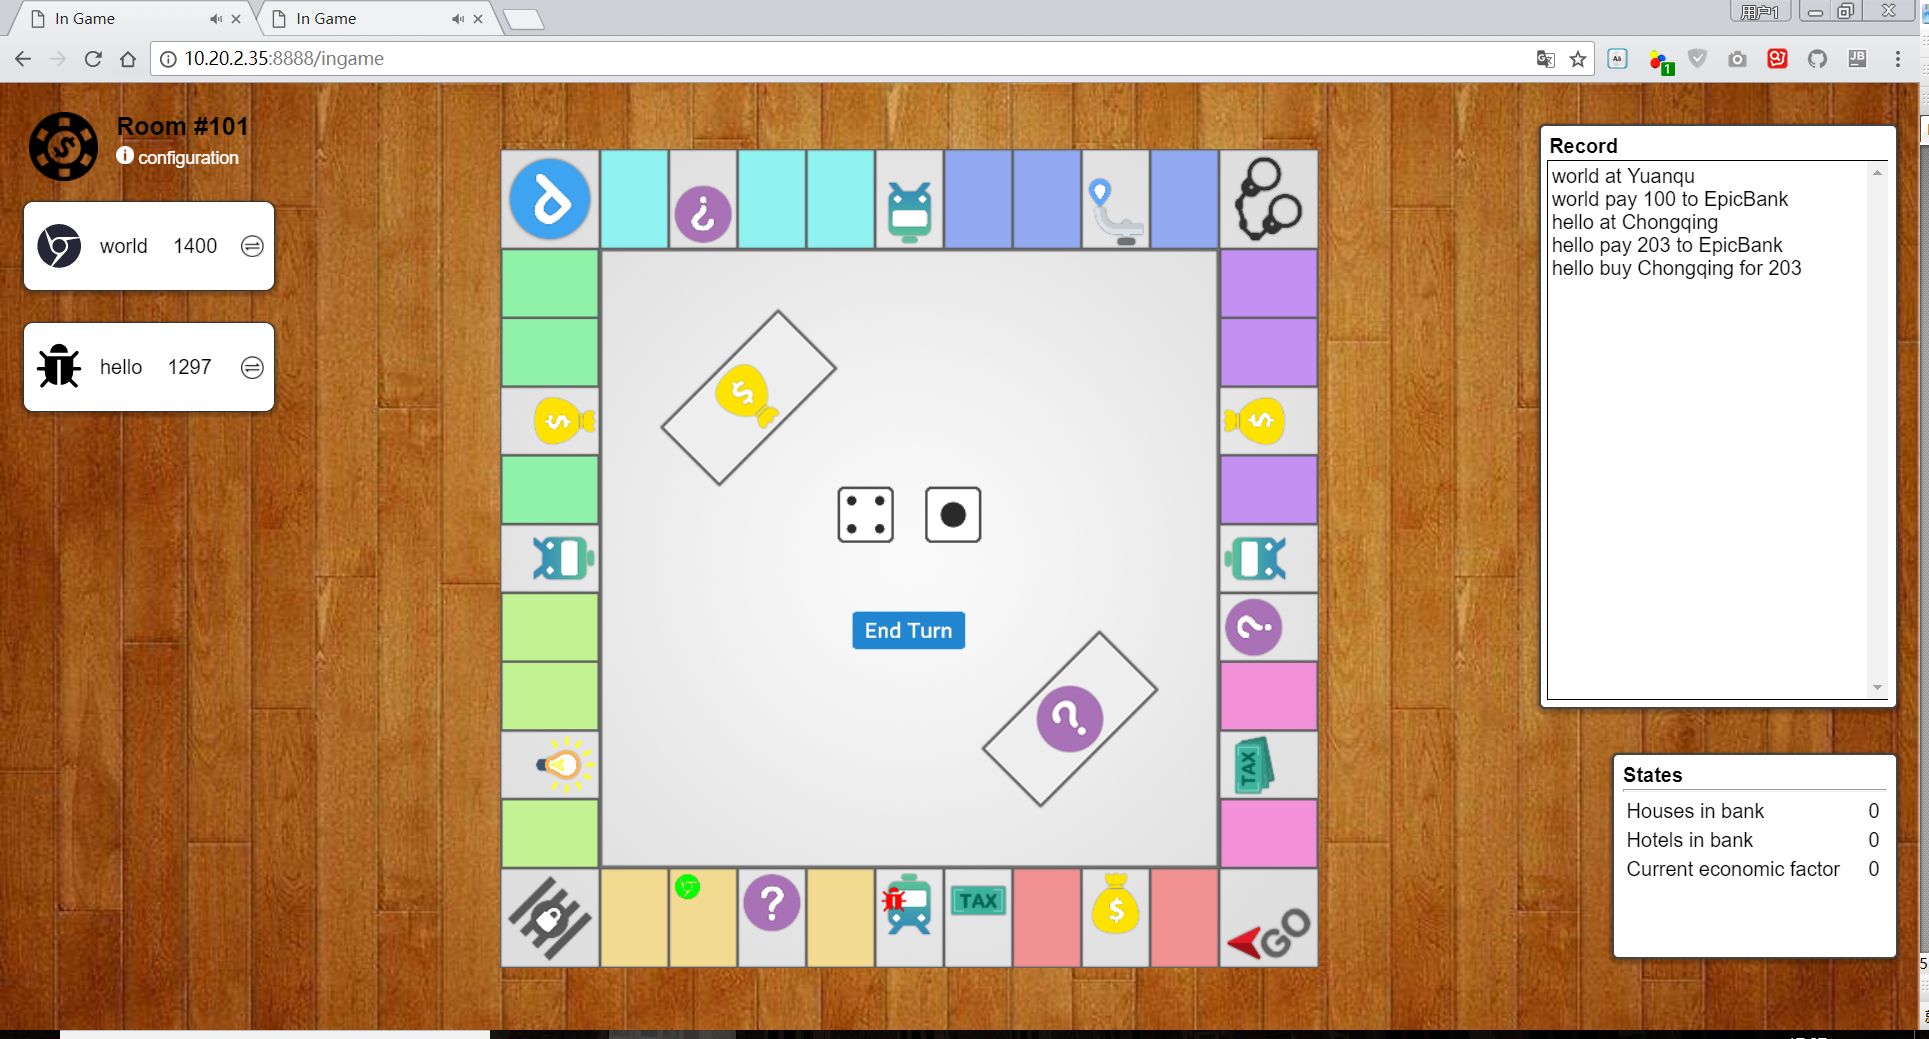
\includegraphics[scale=0.32]{image/ingame3.png}
\caption{Main page 2}
\end{figure}
\begin{figure}[H]
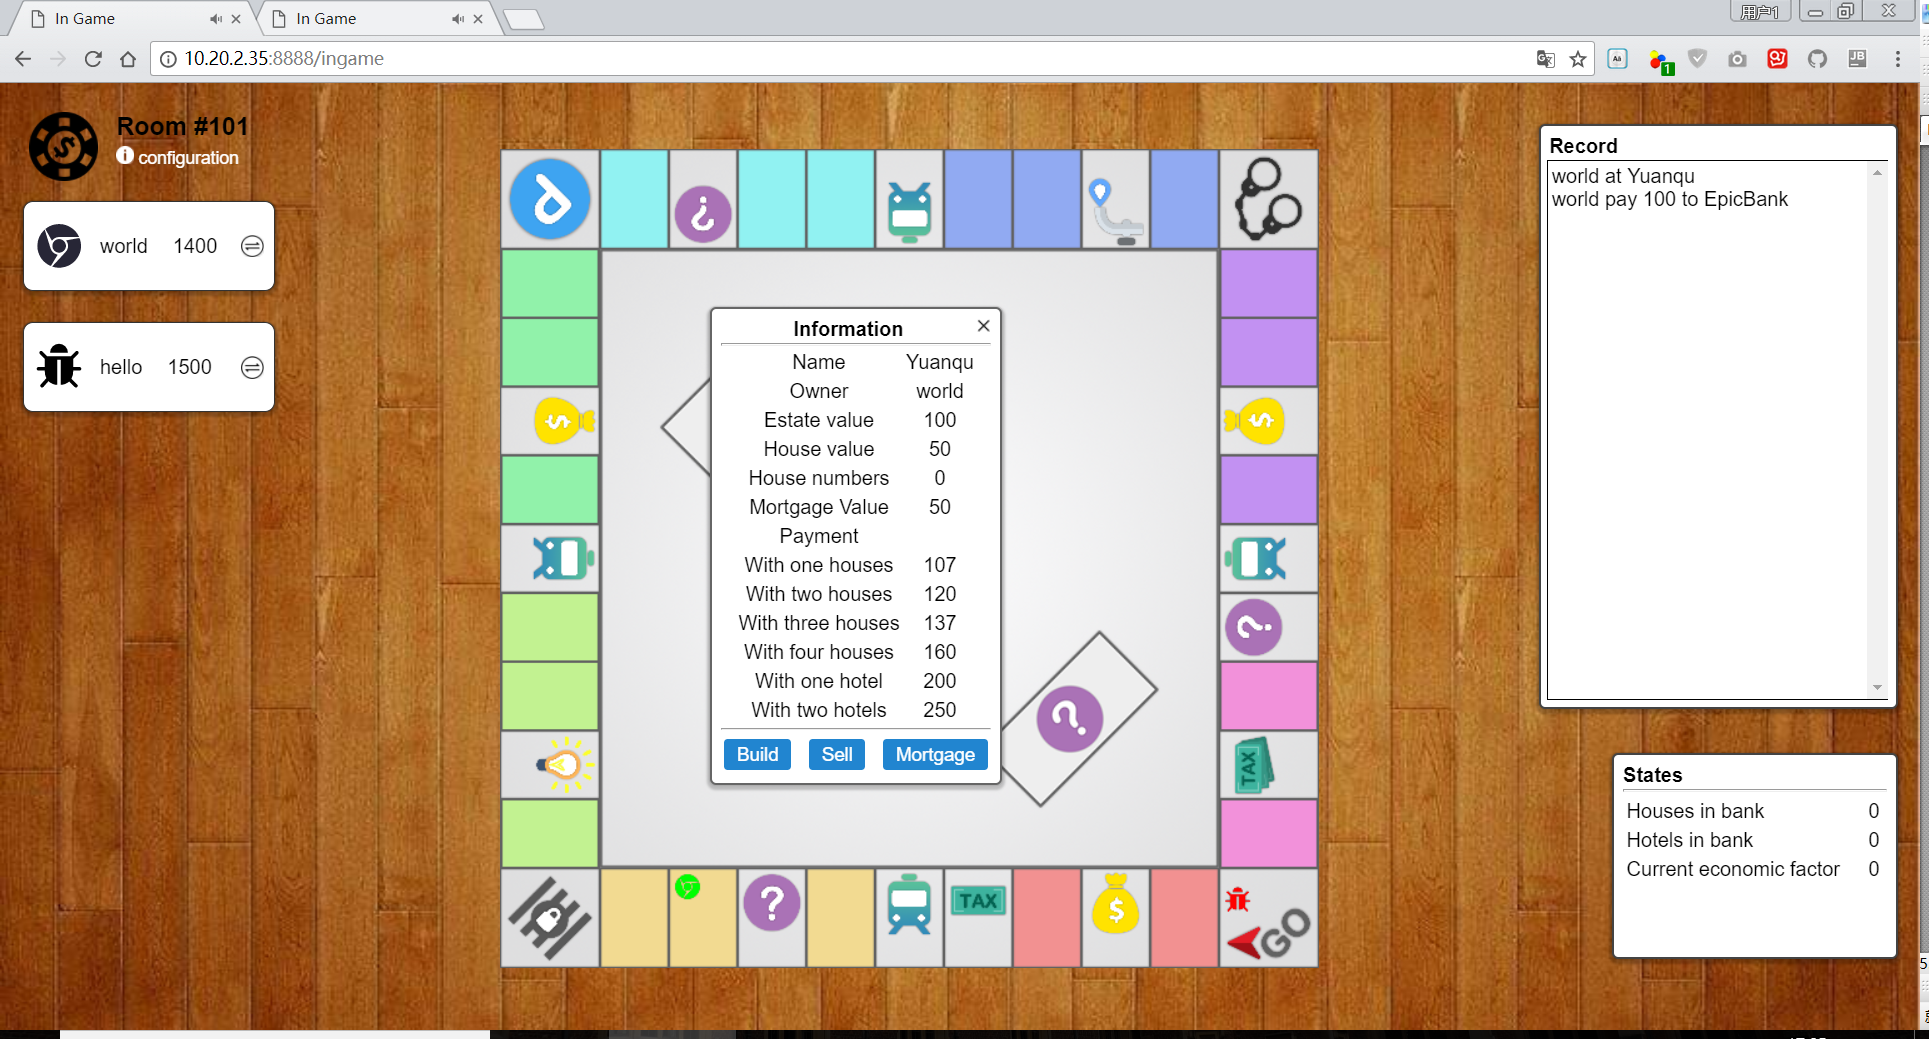
\includegraphics[scale=0.32]{image/ingame2.png}
\caption{Management page}
\end{figure}
\begin{figure}[H]
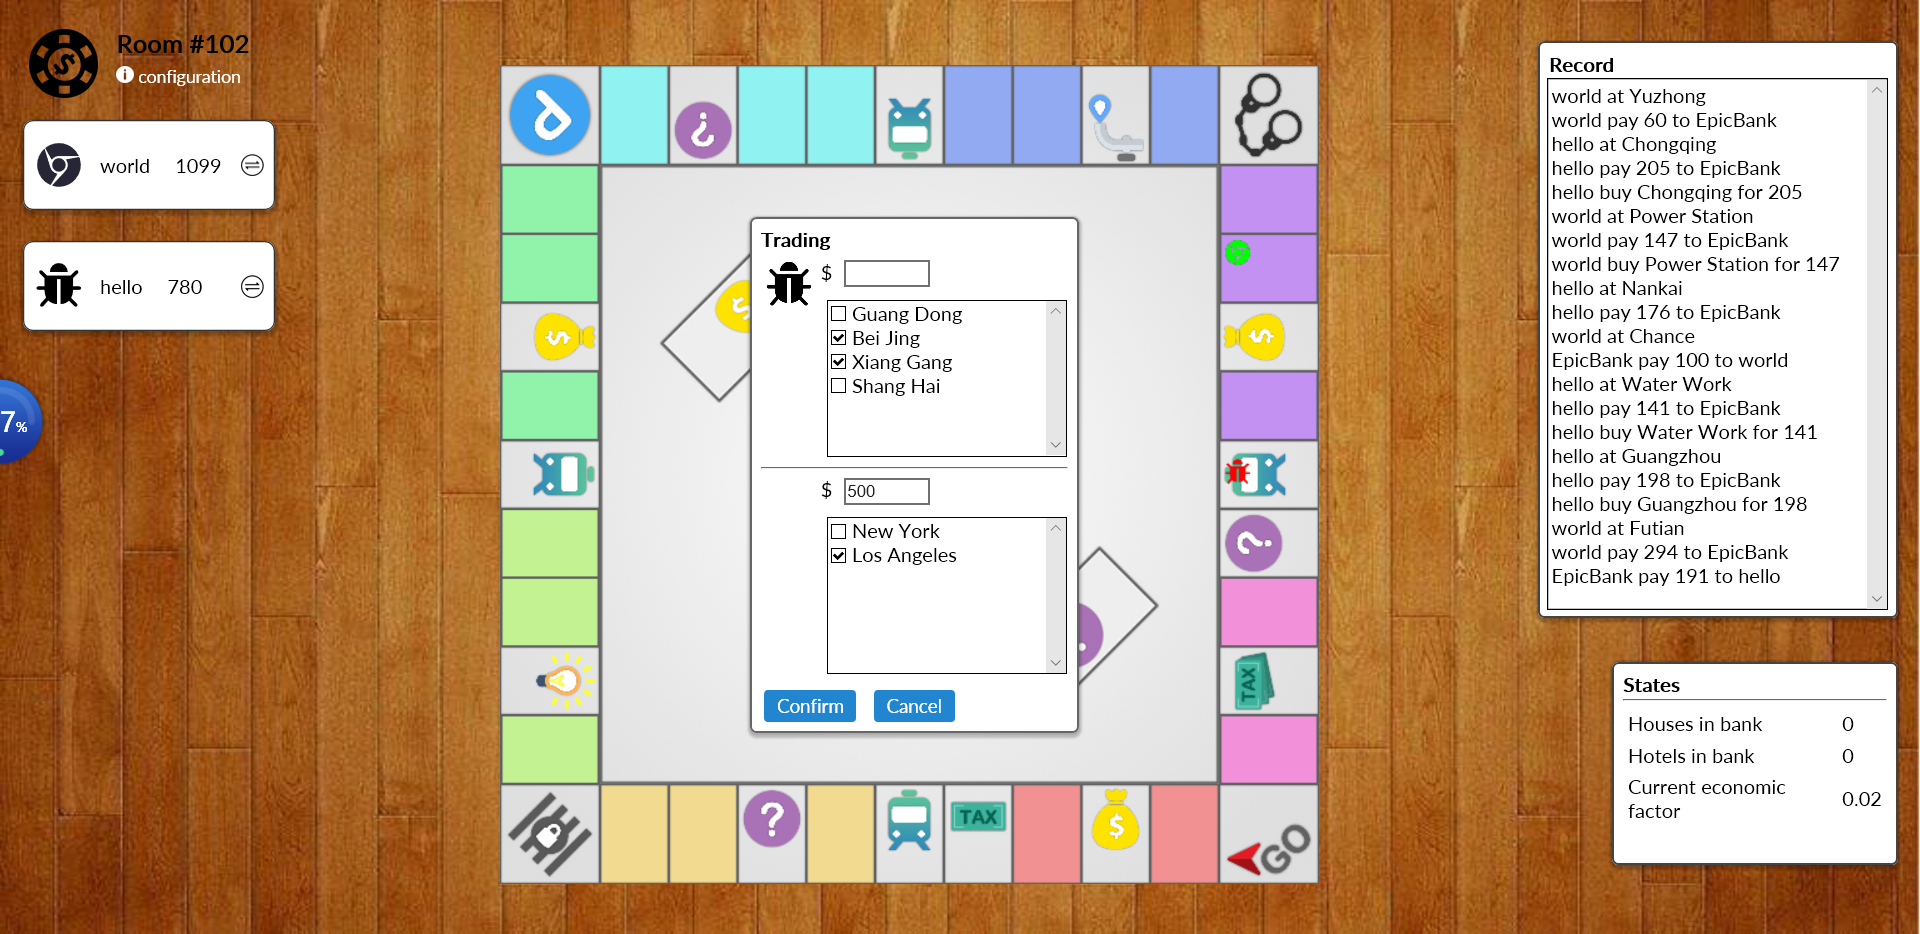
\includegraphics[scale=0.20]{image/trade.png}
\caption{Trade page}
\end{figure}

\end{document}
